% !TEX root = ../thesis.tex

\chapter{Syntactic part}
\label{sec:methodology}
\section{Goal of the work} \label{sec:goal}
Based on the analytical part~\ref{sec:analytical} we will be working on a mathematical models to predict customer behavior consist of vendor, psychology and loyalty sub-models combine in hidden markov model (HMM) to final prediction model.
States in the HMM will be read by viterbi algoritm~\ref{subsec:viterbi} which is able to predict most probability state in propagation by HMM.
We try to get a better results than actual standard statistical methods (Time Series analysis)~\ref{sec:statistics} to predict customer behavior in e-commerce.
In the final our model will be able to predict online store future income from previous income and number of visitors.
For successfully prediction we will use some open data for store strength and customer satisfaction and some predefined and computed variables from store.
\section{Modeling prediction of customer behavior} \label{sec:modeling}
The goal of model is to predict if customer will successfully finish order or leave store without make an order.
This model will be consists of three sub-models.
Vendor model,\ psychology model and loyalty model.
All sub-models will be combined to complex prediction mechanism, as you can see on image~\ref{Model schema with interaction}
To final prediction will be used Hidden Markov model in combination with Viterbi algorithm to detect hidden states to reflect set weights and get better results for each industry.
Weights for model are industry dependent and for my modeling we set them from Megaplay s.r.o data and with cooperation with the owner of Megaplay s.r.o who has more than 10 years of experience in that industry, so he is the right person to know that kind of business.
\\
\begin{figure}[h!]
    \begin{center}
        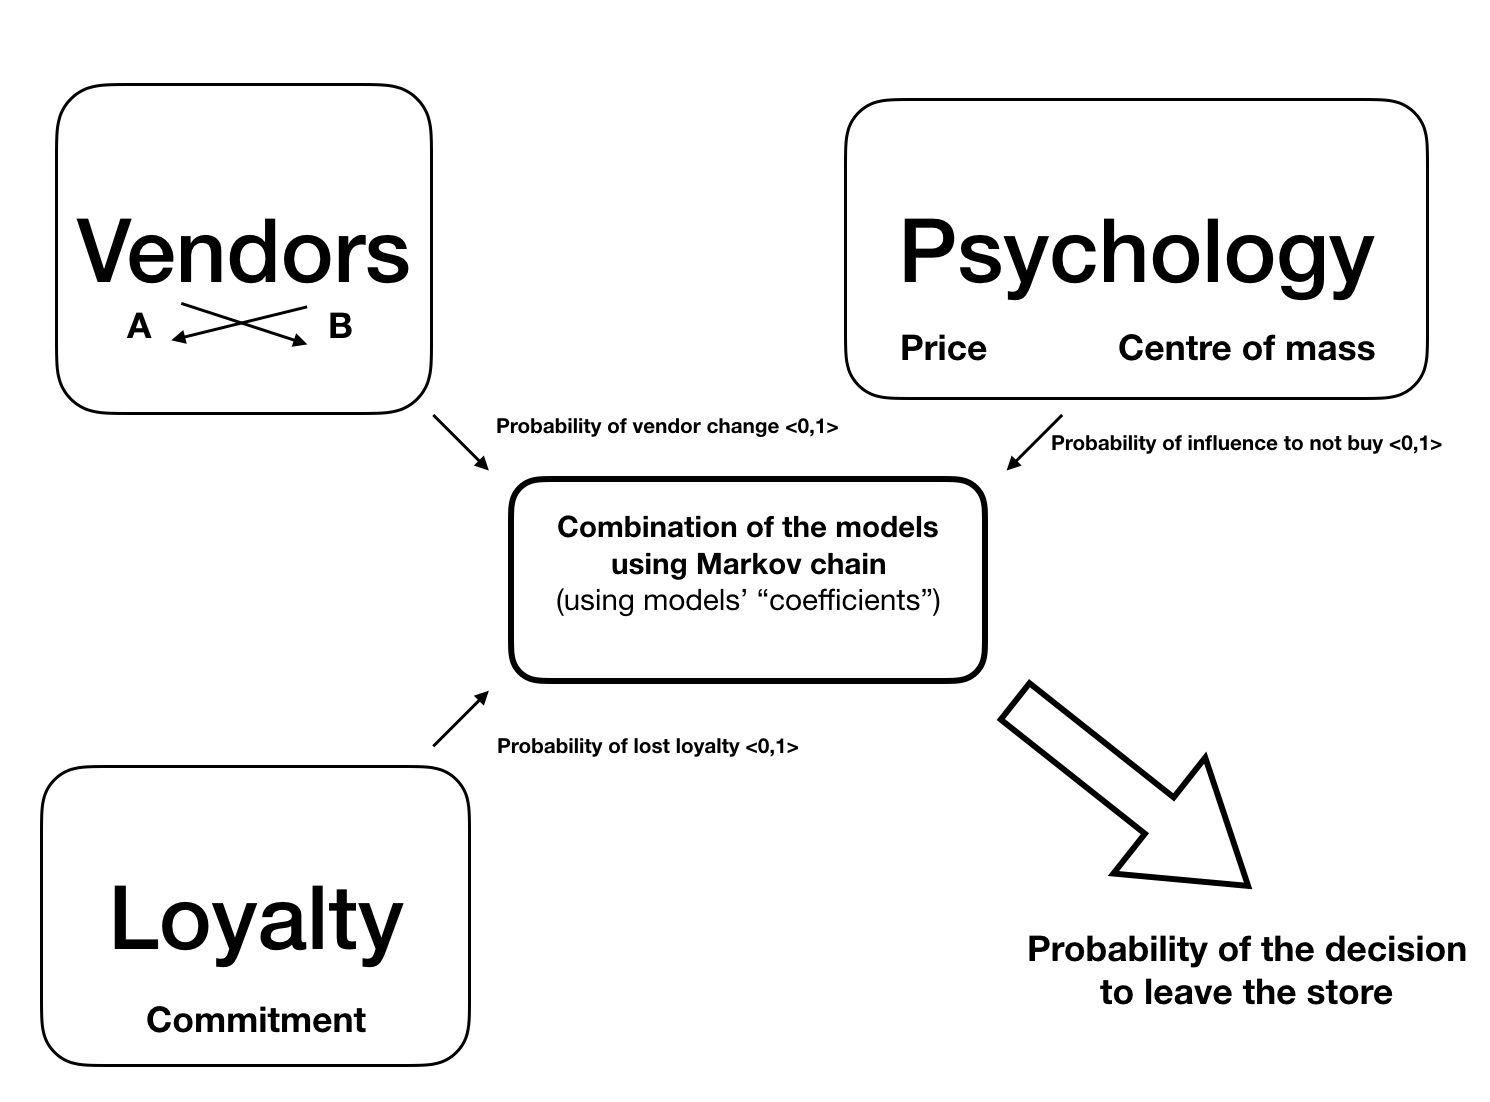
\includegraphics[width=140mm]{computation_schema.png}
    \end{center}
    \caption{Computation flow and interactions between models}
    \label{Model schema with interaction}
\end{figure}
\\
\subsection{Preprocessing of input data} \label{subsec:preprocessing}
Data should have to be anonymize \footnote{Data anonymization is a type of information sanitization whose intent is privacy protection.
It is the process of either encrypting or removing personally identifiable information from data sets, so that
the people whom the data describe remain anonymous.} and pseudonymized \footnote{Pseudonymization is a data management
and de-identification procedure by which personally identifiable information fields within a data record are replaced
by one or more artificial identifiers, or pseudonyms.} to keep legal notice of~\cite{gdpr}.
Then we should utilize data to utilized inputs.
This prepared data I will add to the Matlab live script file to be used for prediction.\\
\\
\textbf{Average day visitors for a predicted month}\\
This value was calculated from anonymize user data from Google Analytics tool used their prediction mechanism to get number of future users based on previous a number of visitors.\\
\\
\textbf{Perceived value for psychology model} \label{perceived}\\
This variable is needed for loyalty model~\ref{subsec:model_loyalty} and comes from an open e-commerce compare data provided by Heureka.cz/Heureka.sk internal tool.\\
\\
\textbf{Number of orders 2018 - 2019}\\
Number of orders get from shopycrm.com tool used in Megaplay s.r.o to manage their business processes and store all needed data.\\
\\
\textbf{Unique products sell}\\
This variable is used in Psychology model~\ref{subsec:model_psychology} for Price aspect calculation~\ref{eq:26}.\\
\\
\textbf{Customer satisfaction} \label{customerSat}\\
This value is provided by Heureka open data, and it's a calculated value from the all customer reviews of the store.\\
\\
\textbf{Margin}\\
The retail margin percentage measures the retail margin as a percentage of the retail price.
This measurement gives you a context for the retail margin.
For example, if you have a 5~€ retail margin on two different products, but one costs 150~€ and next one costs 10~€, the second product would have a much higher retail margin percentage.\\
\\
\textbf{Number of product order each day $Q_i$}\\
This is a calculated value from shopycrm.com about number of product order for each one.
It's used in Psychology model~\ref{subsec:model_psychology}. \\
\\
\textbf{Quality index $Q_1$}\\
This is vendor quality index provided by Heureka open data.
This is a power/strength of the store.
Higher number mean that for a customer is more difficult to leave the store and go to another online store.\\
\\
\textbf{Vendor coefficients $\beta, \gamma, \delta$} \label{vendorCoeff}\\
This three coefficients are used as weight for vendor model~\ref{subsec:model_vendors} and was set with cooperation with Megaplay s.r.o owner for their industry.
It's represent the relation between vendor prices and vendor quality.\\
\\
\begin{table}[h!]
    \begin{center}
        \begin{tabular}{ | l | c |}
            \hline
            {\textbf{Variable name}} & \textbf{Value}\\
            \hline
            average day visitors for a predicted month $U_a$& 2357 \\
            perceived value for psychology model & 0.87 \\
            number of orders 2018 - 2019 $O_c$ & 26 530 \\
            Unique products sell $U_p$ & 11048\\
            Customer satisfaction & 90\%\\
            Margin & 0.27\\
            $Q_i$ & 4.12\\
            $Q_1$ & 0.94\\
            Vendor coefficients: & \\
            $\beta$ & 0.7\\
            $\gamma$ & 0.7\\
            $\delta$ & 0.85\\
            \hline
        \end{tabular}
    \end{center}
    \caption{Coefficient data from Megaplay s.r.o}
    \label{megaplay_data}
\end{table}
\\
\begin{table}[h!]
    \begin{center}
        \begin{tabular}{ | l | c |}
            \hline
            {\textbf{Variable name}} & \textbf{Value equation}\\
            \hline
            number of visitors 1/2020 & $31 * U_a$\\
            average earn per order & $\sum EARN / O_c$\\
            \overline{Q} & $1/U_p * (U_p/ O_c)$\\
            \overline{P} & $1/U_p * margin$\\
            trust & $1/O_c * O_c/U_a$\\
            \hline
        \end{tabular}
    \end{center}
    \caption{Calculated data from Megaplay s.r.o}
    \label{megaplay_data_equation}
\end{table}
\\
\subsection{Vendors} \label{subsec:model_vendors}
For simplification, we will take to account only a two vendors market share, without 100\% domination, because of on a real
market is 100\% monopole unlikely see and then we will be reflected only main competitor.
From that condition it is evident that for market dominate vendor it will return false positive results.
Our model is based on equations from Brands section~\ref{eq:10} and from those equations we will get probability of vendor change from
vendor $A$ to vendor $B$ and if the vendor $B$ will have more strength than vendor $A$ it will break the computation and customer
will leave our store without successfully completing buy process.
Results of this computation wil be probability for each iteration of buy process simulation in an interval $<0,1>$.
Data for this model will comes from open data provided by google.com, heureka.cz/heureka.sk and national governments.
That data will be combined with calculated price indexes downloaded from shopycrm.com tool.
\\
\begin{equation} \label{eq:24}
\alpha_{xy} = \beta H(P_x-P_y) + \gamma H(Qx-Qy) + \delta H(Px-Py)H(Q_x - Q_y)
\end{equation}
\\
where $\beta, \gamma, \delta$ are non-negative~\ref{vendorCoeff}.
\\
\begin{itemize}
    \item $P$ is prices of vendors products
    \item $Q$ is a quality index of vendor
    \item $H$ is a Heaviside function which will be calculated by~\ref{eq:22}.
\end{itemize}
\\
\begin{eqnarray} \label{eq:25}
H(s) = 1, s > 0 \\
H (s) = 0, s \leq 0
\end{eqnarray}
\\
\subsection{Psychology} \label{subsec:model_psychology}
Psychology aspect is trying to simulate customer behavior in thee situation like a prices aspect, society influenced, mood aspect, actual needs
and so on.
In this model we will simplify only for price effect~\ref{subsubsec:model_psychology_price} and center of mass effect~\ref{subsubsec:model_psychology_mass}
\subsubsection{Price aspect} \label{subsubsec:model_psychology_price}
\begin{equation} \label{eq:26}
\overset{-}{Q} = \frac{1}{n_p} \sum_{i=1}^{n_p} Q_i
\end{equation}
\\
\begin{itemize}
    \item $Q_i$ number of orders for product $i$ per day divide amount of orders per same day, prom interval $<0,1>$
    \item $n_p$ number of products in store
\end{itemize}
\\
\begin{equation} \label{eq:27}
\alpha_{ij} = \frac{C+max(Q_j, \overset{-}{Q})}{C+max(Q_i, \overset{-}{Q})}
\end{equation}
\\
Coefficient C is used to be $\alpha_{ij}$ always positive.
\subsubsection{Center of mass aspect} \label{subsubsec:model_psychology_mass}
Center of mass aspect is applied as a part of sociology to our psyhology model.
Marketers use it to manipulate with customers in global way.
Like a black friday, Cyber monday etc., in that days stores manipulate with our psychology by discount prices.
\\
\begin{equation} \label{eq:28}
\overset{-}{P} = \frac{1}{n_p} \sum_{i=1}^{n_p} P_i
\end{equation}
\begin{itemize}
    \item $P_i$ is defined as product price minus retail recommend price divide average price
    \item $n_p$ number of products in store
\end{itemize}
\\
\begin{equation} \label{eq:29}
\alpha_{ij} = \frac{C+max(P_j, \overset{-}{P})}{C+max(P_i, \overset{-}{P})}
\end{equation}
\\
This model returns probability for customer decision to make action from interval $<0,1>$.
\\
\subsection{Loyalty} \label{subsec:model_loyalty}
This models is based on Luarn & Lin research~\cite{luarn} and we change theirs model for our needs.\\
\begin{equation} \label{eq:30}
L = \frac{R+Z}{Z}
\end{equation}
\\
\begin{enumerate}
    \item L ..... probability of whole loyalty model
    \item R ..... probability of separate loyalty model
    \item Z ..... probability of commitment model
\end{enumerate}
\\
As we see on~\ref{Loyalty scheme} Loyalty model is consist of all three sub-models (Trust, Customer Satisfaction, Perceived value)
but commitment model consist of only Trust and Customer Satisfaction.
a,b,c,d,e .... weight coefficient to combine Trust, Customer satisfaction and Perceived value.\\
\newpage
Trust
\begin{equation} \label{eq:31}
T = \frac{1}{n} \sum_{i=1}^{n} O_i
\end{equation}
\\
$O_i$ number of orders divide number of visitors per day $i$
\\
\\
\textbf{Customer satisfaction}~\ref{customerSat} are datasets get from open data per each day, individual satisfaction.
For simplified the situation we will use average satisfaction per whole store.
\textbf{Perceived value}~\ref{perceived} is subjective value, which depend on a strength of the store.
\subsubsection{Commitment and Loyalty} \label{subsubsec:model_loyalty_commitment}
\textbf{Commitment} is making the actual choice every day or other period basis to keep up with something e.g. a relationship, personal goal, a task, etc.
We would have to hold ourself accountable to keep a commitment to something or someone.
Similarly, being loyal involves holding ourself accountable as well.
Against of \textbf{Loyalty} which is usually seen as a character trait rather than a conscious decision.
This model return probability for customer decision to not leave the store from interval $<0,1>$.\\
\\
\begin{figure}[h!]
    \begin{center}
        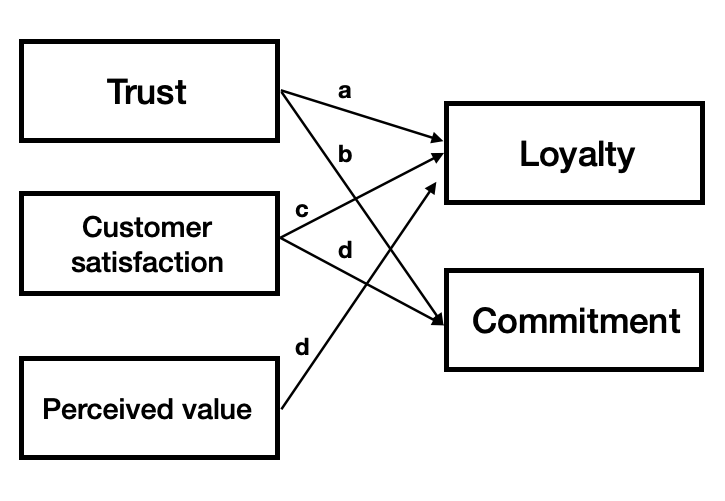
\includegraphics[width=140mm]{loyalty.png}
    \end{center}
    \caption{Computation flow for loyalty and commitment}
    \label{Loyalty scheme}
\end{figure}
\subsection{Combining models to decision process} \label{subsec:combining_models}
All separates models return probabilities vectors which we update to square matrix which is use as input to Hidden Markov model (HMM) \footnote{Hidden Markov Model (HMM) is a statistical Markov model
in which the system being modeled is assumed to be a Markov process with unobservable (i.e. hidden) states.
The hidden Markov model can be represented as the simplest dynamic Bayesian network.
The mathematics behind the HMM were developed by L. E. Baum and coworkers.
HMM is closely related to earlier work on the optimal nonlinear filtering problem by Ruslan L. Stratonovich,
who was the first to describe the forward-backward procedure.}
These probabilities will be combined with specific weights coefficients to always prevent positives results.
\section{Decision process from sub-models} \label{sec:decision}
\subsection{Hidden markov model} \label{subsec:hhm}
In a Hidden Markov Model (HMM), we have an invisible Markov chain (which we cannot observe), and each state
generates in random one out of $k$ observations, which are visible to us. Let’s look at an example.
Suppose we have the Markov Chain from above, with three states (snow, rain and sunshine),
$P$ - the transition probability matrix and $q$ — the initial probabilities.
This is the invisible Markov Chain — suppose we are home and cannot see the weather.
We can, however, feel the temperature inside our room, and suppose there are two possible observations: hot and cold.\\
For our need we will create 3 states model.
States will be:\\
\begin{itemize}
    \item order
    \item not finished order
    \item no order decision
\end{itemize}
With Megaplay s.r.o owner and heureka e-comerce tool calculation data we were set probability wages vector for HMM function like:\\
$$ p_w = \left(\frac{1}{3} & \frac{1}{2} & \frac{1}{9}\right) $$
\\
Vector have to be updated to square matrix which is used in HMM function.\\
\begin{equation*}
    P_w =
    \begin{pmatrix}
        \frac{1}{3} & \frac{1}{2} & \frac{1}{9} \\
        \frac{1}{3} & \frac{1}{2} & \frac{1}{9} \\
        \frac{1}{3} & \frac{1}{2} & \frac{1}{9}
    \end{pmatrix}
\end{equation*}\\
\\
\subsection{Used software, libraries and predefined functions} \label{subsec:libraries}
\textbf{Matlab 2020a}\\
MATLAB (matrix laboratory) is a fourth-generation high-level programming language and interactive environment for numerical
computation, visualization and programming developed by MathWorks.\\
\\
\textbf{Matlab LiveScript}~\cite{livescript}\\
MATLAB live scripts and live functions are interactive documents that combine MATLAB code with formatted text, equations,
and images in a single environment called the Live Editor.
In addition, live scripts store and display output alongside the code that creates it.\\
Use live scripts and functions to:\\
\begin{itemize}
    \item Visually explore and analyze problems
    \item Share richly formatted, executable narratives
    \item Create interactive lectures for teaching
\end{itemize}\\
\\
\textbf{hhmgenerate}~\cite{hhmgenerate}\\
The function $hmmgenerate$ begins with the model in state 1 at step 0, prior to the first emission.
The model then makes a transition to state $i_1$, with probability $T_{1i_1}$, and generates an emission $a_k_1$ with probability $E_{i_1k_11}$.
$hmmgenerate$ returns $i_1$ as the first entry of states, and $a_k_1$ as the first entry of seq.
$[seq,states] = hmmgenerate(len,TRANS,EMIS)$ takes a known Markov model, specified by transition probability matrix $TRANS$ and emission probability matrix $EMIS$,
and uses it to generate:\\
\begin{itemize}
    \item A random sequence seq of emission symbols
    \item A random sequence states of states
\end{itemize}
The length of both $seq$ and $states$ is $len$.
$TRANS(i,j)$ is the probability of transition from state $i$ to state $j$.
$EMIS(k,l)$ is the probability that symbol $l$ is emitted from state $k$.\\
\\
\textbf{hhmviterbi}~\cite{hhmviterbi}\\
The function $hmmviterbi$ begins with the model in state 1 at step 0, prior to the first emission.
hmmviterbi computes the most likely path based on the fact that the model begins in state 1.
$STATES = hmmviterbi(seq,TRANS,EMIS)$ given a $sequence, seq$, calculates the most likely path through the hidden Markov model
specified by transition probability matrix, $TRANS$, and emission probability matrix $EMIS$. $TRANS(i,j)$ is the probability of transition from state $i$ to state $j$.
$EMIS(i,k)$ is the probability that symbol $k$ is emitted from state $i$.\\
\\
\textbf{shopycrm.com}\\
Online CRM application focused on e-commerce stores which provides all store workflows and get precalculated data which we will use for our models to simplify the prediction calculation.
\newpage
\section{Time series for setting reference values} \label{sec:timeseries}
Based on statistical solution chapter~\ref{sec:statistics} we create four statistical approaches to predict 1/2020 income for store based on previous data from years 2018 and 2019.
This previous income can be found in appendix A Reference data~\ref{reference_data}.
To have a better idea about a point of view look on graph~\ref{income} with income data.\\
\begin{figure}[h!]
    \begin{center}
        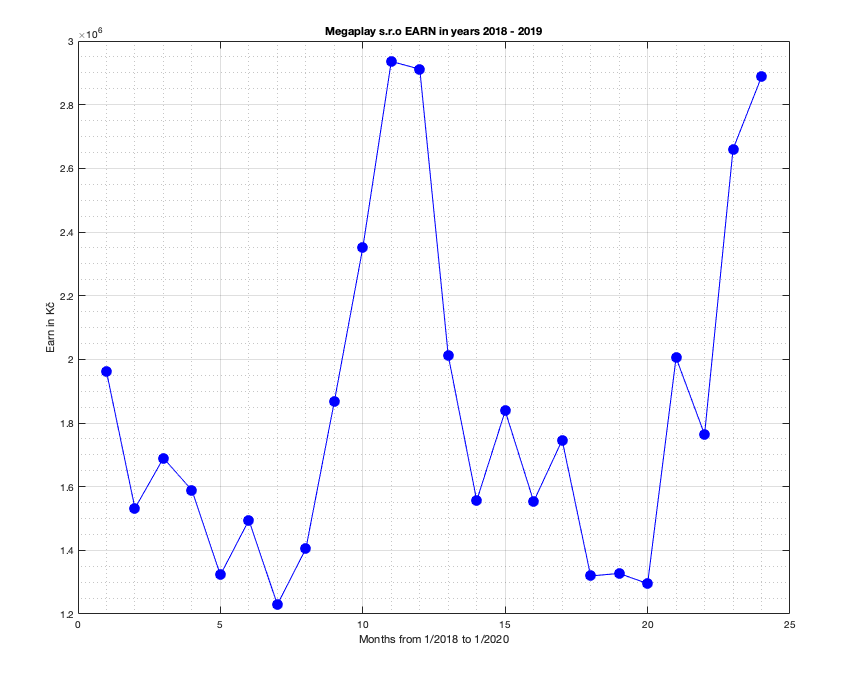
\includegraphics[width=150mm]{income.png}
    \end{center}
    \caption{Megaplay s.r.o income from stores in 2018 - 2019}
    \label{income}
\end{figure}
\subsubsection{Moving average}
Like a first basic time series analysis we tried moving averages.
This method looks like not useful for our needs, because of not able to reflecting trend in
specific e-commerce trends as Christmas time and new years discounts.
For our prediction reference data we will create prediction with moving average $n=3$ and $n=5$.
Here you can see part of code in Matlab to create the prediction, than you can see results in graph~\ref{moving_average_3}
for $n=3$ and on the next graph~\ref{} for $n=5$\\
\\
\textbf{Calculation for n=3}\\
\begin{lstlisting}[language=mcode]
% generate matrix for moving average n=3
% EARN is matrix with income data per months
for i = 2:length(EARN)
    if i < 24
        average3(1,i-1) = (EARN(1, i-1)+EARN(1, i)+EARN(1,i+1))/3;
    end
end

% with wages 1/4 1/2 1/4
for i = 2:length(EARN)
    if i < 24
        average3wages(1,i-1) = (1/4*EARN(1, i-1))+ ...
        (1/2*EARN(1, i))+(1/4*EARN(1,i+1));
    end
end

% moving average n=3 first level prediction
firstLevelPrediction = 1/3*(-2*EARN(1,22)+1*EARN(1,23)+4*EARN(1,24))
\end{lstlisting}\\
\\
Result from this prediction for 1/2020 is 3 561 213 Kč and it's aberration is 41.88\%.\\
\\
\textbf{Calculation for n=5}\\
\begin{lstlisting}[language=mcode]
% generate matrix for moving average n=5
% EARN is matrix with income data per months
for i = 3:length(EARN)
    if i < 23
        average5(1,i-2) = (EARN(1, i-2)+EARN(1, i-1)+EARN(1, i)+ ...
        EARN(1,i+1)+EARN(1, i+2))/5;
    end
end

% with wages 1/35(-3,12,17,12,-3)

for i = 3:length(EARN)
    if i < 23
        average5wages(1,i-2) = 1/35*(-3*EARN(1, i-2)+ ...
        12*EARN(1, i-1)+17*EARN(1, i)+12*EARN(1, i+1)-3*EARN(1, i+2));
    end
end

% first level prediction for n=5
firstLevelPrediction5 = 1/10*(-4*EARN(1,20)-1*EARN(1,21)+...
                        2*EARN(1,22)+5*EARN(1,23)+8*EARN(1,24))
% second level prediction for n=5
secondLevelPrediction5 = 1/5*(3*EARN(1,20)-3*EARN(1,21)-...
                        4*EARN(1,22)+0*EARN(1,23)+9*EARN(1,24))
\end{lstlisting}\\
\\
Result from this prediction for 1/2020 are 3 274 399 Kč and it's aberration is 33.91\% for first level prediction and 3 361 156 Kč with aberration 30.45\%.\\
\begin{figure}[h!]
    \begin{center}
        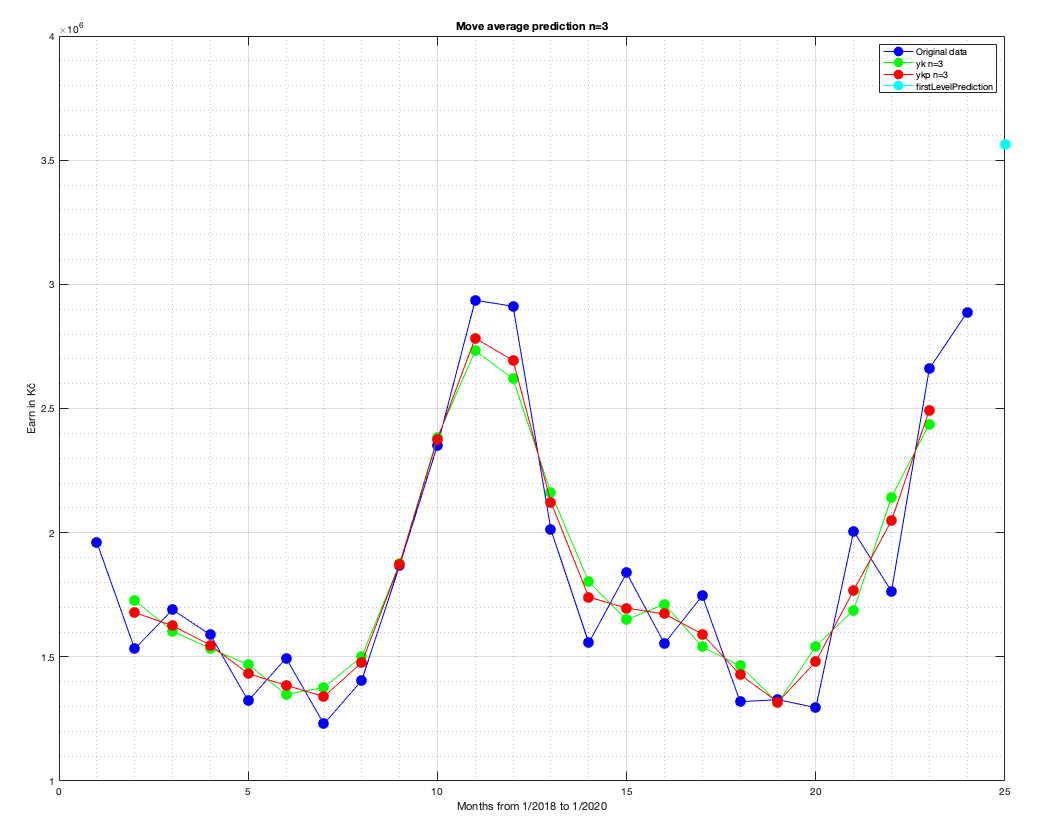
\includegraphics[width=150mm]{moving_average_3.png}
    \end{center}
    \caption{Moving average results for n=3}
    \label{moving_average_3}
\end{figure}
\begin{figure}[h!]
    \begin{center}
        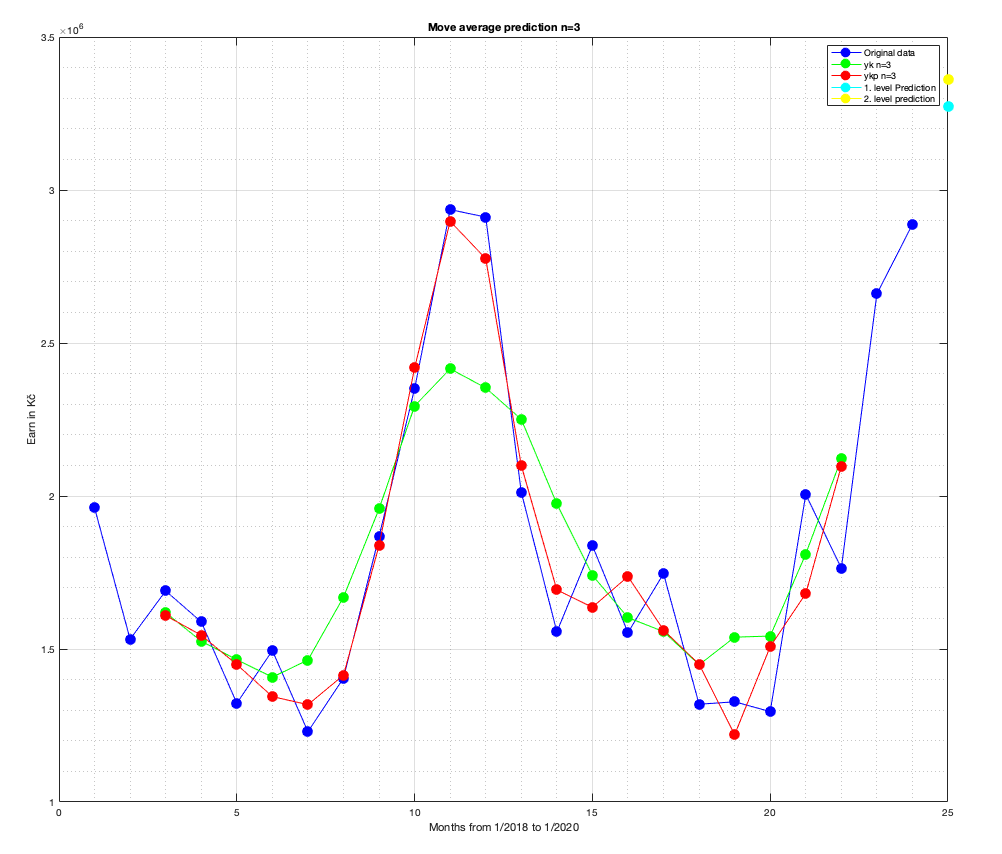
\includegraphics[width=150mm]{moving_average_5.png}
    \end{center}
    \caption{Moving average results for n=5}
    \label{moving_average_5}
\end{figure}
\subsubsection{Models}
After moving average we use two models for linear regression to predict other reference data by better statistical solutions.
We will use these two models:
\begin{itemize}
    \item $Tr_{t1}=a_0+a_1t$
    \item $Tr_{t2}=a_0+a_1t+a_2t^2$
\end{itemize}\\
\\
\textbf{Regression analysis for $Tr_{t1}=a_0+a_1t$}\\
\begin{lstlisting}[language=mcode]
X = [ones(1,24); ...
1:1:24];
XTX = X*X';
invXTX = inv(XTX);
XTY = X*EARN';
parameters = invXTX*XTY;
a0 = parameters(1, 1);
a1 = parameters(2, 1);
Trt1 = a0+a1.*t;

%prediction for 1/2021
PredictionTrt1 = a0+a1*25
\end{lstlisting}\\
\\
\textbf{Regression analysis for $Tr_{t2}=a_0+a_1t+a_2t^2$}\\
\begin{lstlisting}[language=mcode]
X2 = [ones(1,24); ...
    1:1:24; ...
    1^2 2^2 3^2 4^2 5^2 6^2 7^2 ...
    8^2 9^2 10^2 11^2 12^2 13^2 14^2 15^2 16^2 ...
    17^2 18^2 19^2 20^2 21^2 22^2 23^2 24^2];
XTX2 = X2*X2';
invXTX2 = inv(XTX2);
XTY2 = X2*EARN';
parameters = invXTX2*XTY2;
a0 = parameters(1, 1);
a1 = parameters(2, 1);
a2 = parameters(3, 1);
Trt2 = a0+a1.*t+a2.*t.^2;

%prediction for 1/2020
PredictionTrt2 = a0+a1*25+a2*25^2
\end{lstlisting}\\
\\
We got better results from model $Tr_{t2}=a_0+a_1t+a_2t^2$ as you can see on graph~\ref{ts_models}.
The goal of this thesis is not about to find the best statistical solutions in time series, so for our purpose this model is enough as a reference.
Time series analysis for better model have the results with aberration of 14,56\% from the real 2020 income.
All models result you can see in evaluation part~\ref{evaluation}.\\
\begin{figure}[h!]
    \begin{center}
        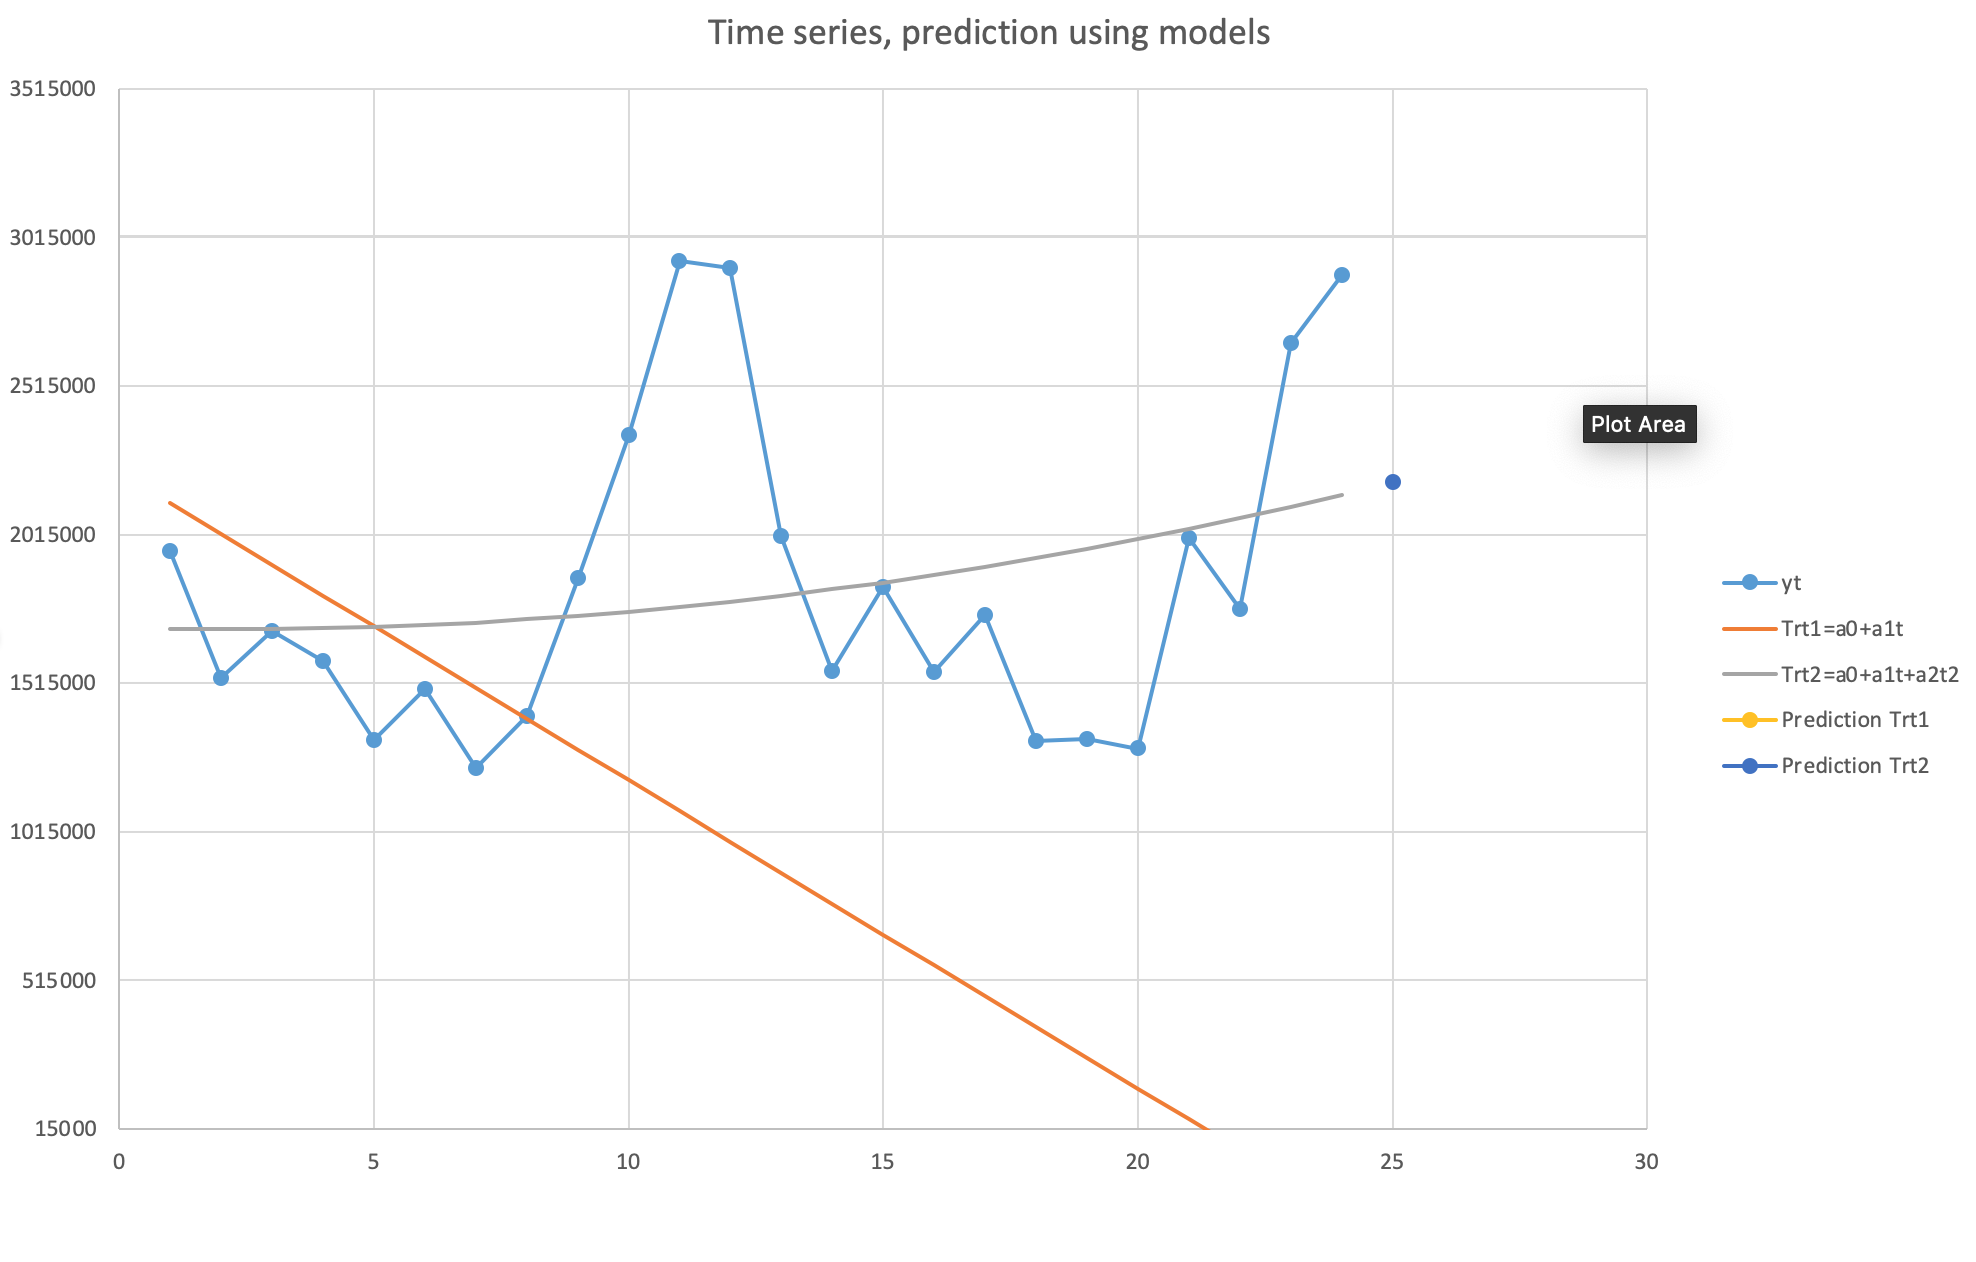
\includegraphics[width=140mm]{model_ts.png}
    \end{center}
    \caption{Time series model results}
    \label{ts_models}
\end{figure}
\newpage
\section{Prediction application} \label{sec:app}
Our prediction script is finally written in Matlab Live script with predefined constants based on Megaplay s.r.o data,
but for modeling and dynamic prediction are used Live scripts Controls so in the script we are able to easily set all constant to model for simulate different situations. We can see model situation in~\ref{appendixc} and taht results is described in the final summary~\ref{summary}.\\
\subsection{Using random values} \label{subsec:rand}
In our model we use random generated variables to simulate situations from real store where the user can compare with other store in the different situation.
This other stores and situation should be better or worst to actual store.
\subsection{Main Matlab code} \label{subsec:matlab}
\begin{lstlisting}[language=mcode]
% generate 10 times for get average values to prevent
% false positive and negative results
for c=1:experimentationCycles
    % go with each visitor thrue the prediction model and get
    for i=1:numberOfVisitors1_2020
        % actual tested value for each cycle
        Pj = generatePriceOfProduct();
        % product price minus product retail price
        Pi = Pj*margin;
        % actual product order value for each cycle
        Qj = 1;
        % statistic value get from open data
        if rand(1) > 0.98
            % Quality index for vendor 2
            Q2 = Q1 - rand(1);
            % vendor 2 product price
            P2 = Pj  - rand(1);
            satisfaction = customerSatisfaction - randi(10);
        else
            % Quality index for vendor 2
            Q2 = Q1 + rand(1);
            % vendor 2 product price
            P2 = Pj + rand(1);
            satisfaction = customerSatisfaction+randi(10);
        end
        % get value of vendor submodel
        vendorProbability = vendor(beta, gamma, delta,...
                            Pj, P2, Q1, Q2);
        % get value of psychology submodel
        psychologyProbability = psychology(averageP,...
                averageQ,Pj, Pi, Qj, Qi);
        % get value of loyalty submodel
        loyaltyProbability = loyalty(satisfaction,...
                trust, perceived);
        % customer goes to other online store
        % go to next cycle
        if vendorProbability == 0
            continue
        end

        % prepare square matrix for hidden markov model
        trans = [vendorProbability vendorProbability ...
        vendorProbability; psychologyProbability ...
        psychologyProbability psychologyProbability; ...
        loyaltyProbability loyaltyProbability ...
        loyaltyProbability];

        % generate hidden markov model data
        [seq,states] = ...
            hmmgenerate(3,trans,probabilityWages,...
                'Statenames',{'order';'not finished order';...
                'no order decision'});

        % use viterbi algoritm to get states during hmm
        estimatesStates = ...
            hmmviterbi(seq,trans,probabilityWages,...
                'Statenames',{'order';'not finished order';...
                'no order decision'});

        % check states that customer not finished order
        exactMatchMask = strcmp(estimatesStates,...
                'no order decision');

        if  sum(exactMatchMask) < 1
            orders = orders + 1;
            % increate psychology effect of success store
            % when order is finished
            Qj = Qj + 1;
        end
    end
end
\end{lstlisting}\\
\subsection{Sub-models function in Matlab} \label{subsec:matlab-sub-models}
\begin{lstlisting}[language=mcode]
% model for calculation vendor probability
function v = vendor(beta, gamma, delta, Px, Py, Qx, Qy)
    v = (beta * heaviside(Px - Py))+(gamma * heaviside(Qx-Qy))+...
        (delta * heaviside(Px - Py) * heaviside(Qx-Qy));
end

% model for cacluclation loaylty probability
function l = loyalty(satisfaction, trust, percieved)
    R = satisfaction + trust + percieved;
    Z = trust + satisfaction;
    l = (R + Z) / Z;
end

% model for calculation psychology probablity
function p = psychology(averageQ, averageP, Pj, Pi, Qj, Qi)
    p = (1 + max(Pj, averageP) / 1 + max(Pi, averageP)) + ...
        (1 + max(Qj, averageQ) / 1 + max(Qi, averageQ));
end

% generate random value of order
function price = generatePriceOfProduct(min, max)
    price = (max-min).*rand(1) + min;
end
\end{lstlisting}\\
